\documentclass[14pt]{article}
\usepackage[utf8]{inputenc}
\usepackage[english,russian]{babel}
\inputencoding{utf8}
\usepackage{graphicx}
\usepackage{amsfonts}
\usepackage{amsmath}
\usepackage{amssymb}
\usepackage{indentfirst}
\usepackage{epsfig}
\usepackage{ccaption}
\textwidth 16.5cm
\textheight 22cm
\voffset=-1.4cm
\hoffset=-2.3cm

\title{\bf Определение параметров межзвездного поглощения света по данным каталога Hipparcos}

\begin{document}
    \maketitle
    
    \section{Абстракт}
    		Основная задача исследования – автоматический поиск пылевых облаков в окрестности Солнца на основе массовых каталогов звезд. Первый этап этой задачи – построение двумерной панорамы распределения пылевых облаков на небесной сфере на основе данных каталога Hipparcos. Метод исследования основан на сравнении эталонного показателя цвета звезды данного спектрального класса с наблюдаемым показателем цвета. Так как полная двумерная спектральная классификация известна не для всех звезд каталога Hipparcos, то пришлось решать вспомогательную задачу: используя параллаксы звезд каталога Hipparcos дополнить информацию о звездах классом светимости на основе данных о видимой звездной величине и параллаксе звезды. Для этого использовался метод опорных векторов. В результате работы была построена карта распределения пылевой материи, вызывающей покраснения света звезд, по небесной сфере. Для построения трехмерного распределения пылевых облаков необходим более точный и массовый каталог параллаксов звезд, которым может стать каталог миссии GAIA, завершение которой планируется в ближайшие годы.
    
    \section{Постановка задачи}
        {\it Покраснение} света от звезды есть
        $$
            E = E_{B - V} = (B - V)_{obs} - (B - V)_{int}    
        $$ 
        Где $(B - V)_{obs}$ --- ее видимый нами показатель цвета, а $(B - V)_{int}$ --- реальный показатель цвета звезды. Существуют таблицы <<спектральный класс --- показатель цвета>>, поэтому для каждой звезды из каталога Hipparcos, у которой есть видимый показатель цвета и спектральный класс, можно вычислить покраснение. Если мы для всех таких звезд знаем еще и их пространственные координаты с хорошей точностью, то мы можем говорить о пространственном распределении покраснения. В данной работе мы рассмотрим это распределение с точки зрения трендов покраснения в различных направлениях. Результатом работы будут коэффициенты $a$ и $b$ этих трендов $ar + b$. 
        
    \section{Обзор литературы}
        Этот раздел еще не создан
        
    \section{Недостатки используемых методов}
        Этот раздел еще не создан
        
    \section{Метод нахождения параметров межзвездного поглощения}
    
        Нижеописанный метод состоит из трех этапов
    
        \subsection{Картирование небесной сферы}
            Для картирования небесной сферы мы воспользуемся стандартным алгоритмом Healpix, с помощью которого мы разобьем сферу на достаточно маленькие равновеликие части. Назовем их $\{P_i\}_{i = 1}^{2n^2}$ (у нас $n = 18$). Обозначим конусы, высекаемые соответствующими частями через $\{C_i\}_{i = 1}^{2n^2}$\\
        
            Такое разбиение позволит нам,
            \begin{enumerate}
                \item Рассмотреть ход покраснения в каждом конусе как одномерную функцию $E(r)$. Это корректно, ввиду того, что конусы достаточно узкие;
                \item Сделать наши результаты <<независимыми>>, т.к. конусы не налагаются;
                \item Поместить в каждый конус примерно одинаковое число звезд, чтобы избежать недостатка звезд в некоторых конусах.  
            \end{enumerate}      
            
        \subsection{Тренд}
            Тем самым, мы ищем $E_i(r)$, соответствующую каждому $C_i$. Ввиду того, что практически все $E_i(r)$ очень сильно зашумлены разного рода ошибками, не удается проследить истинный ход этих функций. Но тренд все же можно вычислить. Он находится с помощью метода наименьших квадратов.  
            
        \subsection{Критерии выбора звезд}
            \subsubsection{По параллаксу}
                В каталоге Hipparcos, далекие звезды имеют очень большие ошибки в параллаксе. На расстояниях, скажем, в 400 пк эти ошибки могут достигать 100\%. Такие ошибки могут очень сильно испортить наши результаты. Тем самым, мы не будем рассматривать звезды, у которых параллакс (его среднее значение) превосходит 300 пк. Меньшее значение порога оставит нам очень малое число звезд, которых не хватит для того, чтобы вычисленные тренды были достоверными.
            \subsubsection{По тренду}
                Покраснения некоторые звезд очень сильно портят тренды. Иногда они даже бывают отрицательными, что вообще противоречит здравому смыслу. Но об этом мы поговорим позже.
                
                Как известно, метод наименьших квадратов не устойчив к выбросам, т.е. совсем неверные покраснение/параллакс могут очень сильно испортить тренд. Это пример $E(r)$ и тренда в одном из конусов, 
                \begin{center}
                    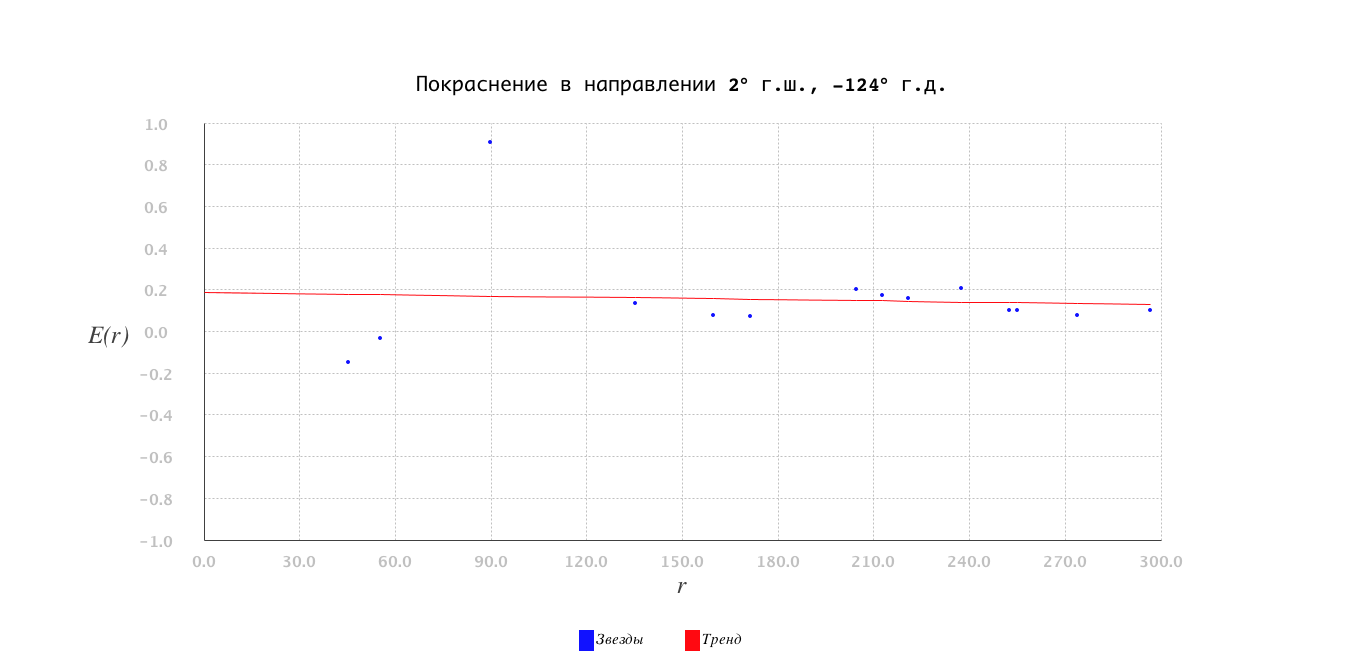
\includegraphics[scale=0.35]{ls.png}
                \end{center}
                
                На этом графике видно, как аномальное значение покраснения звезды (той, что сверху) <<приподнимает>> начало тренда.
                
                
                Для устойчивого построения тренда, мы воспользуемся первой итерацией метода RANSAC. Она заключается в том, что после построения тренда по всем звездам, мы выбрасываем те, у которых отклонение от тренда самое большое. Затем, мы строим тренд заново, но уже только по оставшимся звездам. В методе RANSAC эта процедура выполняется много раз, но нам это не подойдет, т.к. тогда мы будем заниматься <<подгонкой>>. После выброса 10\% самых плохих звезд тренд в том же конусе становится таким,
                \begin{center}
                    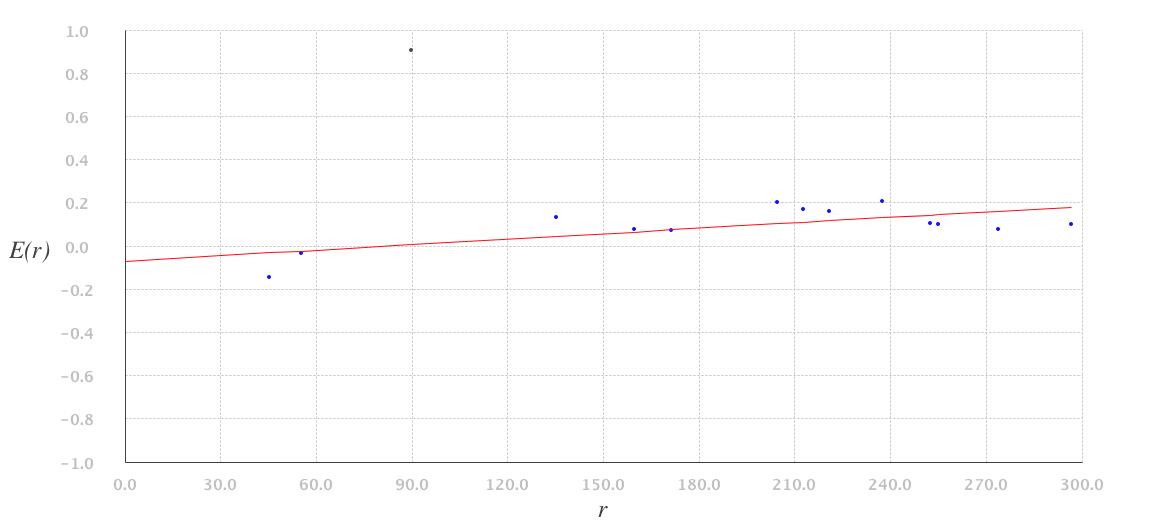
\includegraphics[scale=0.4]{ransac.png}
                \end{center} 
                
                Что чуть больше похоже на правду. В данном случае, мы выбросили одну звезду. 10\% звезд --- это 0, 1, 2 звезды в каждом конусе. Опять же, нельзя выкидывать слишком много звезд из-за опасности <<подгонки>> модели.     
                
        \subsection{}
            Подитожим все вышесказанное. Составим алгоритм расчета             
                
    

    
\end{document}